% Problem 3/7 solution
\noindent
\underline{Solution:}\\

\noindent
First we construct the secular equation (matrix form) corresponding to the 
H\"uckel approximation:\\

$$\begin{pmatrix}
\alpha - E & \beta & 0\\
\beta & \alpha - E & \beta\\
0 & \beta & \alpha - E\\
\end{pmatrix}
\begin{pmatrix}
c_1\\
c_2\\
c_3\\
\end{pmatrix}
= 0$$

\noindent
Denote $x = (\alpha - E) / \beta$ and recall this set of equations
has a non-trivial solution only if the corresponding determinant is zero:

$$\begin{vmatrix}
x & 1 & 0\\
1 & x & 1\\
0 & 1 & x\\
\end{vmatrix}
= 0$$

\noindent
By expanding this determinant, we get:

$$x(x^2 - 1) - x = x^3 - 2x = x(x^2 - 2) = 0 \Rightarrow x =
\left\{
\begin{matrix}
0\\
+\sqrt{2}\\
-\sqrt{2}\\
\end{matrix}
\right.
$$

$$\Rightarrow E = \left\{\begin{matrix}
\alpha\\
\alpha - \sqrt{2}\beta\\
\alpha + \sqrt{2}\beta\\
\end{matrix}\right.
$$

\noindent
Thus we have the following energetics for the orbitals:

\begin{figure}[h]
\centering
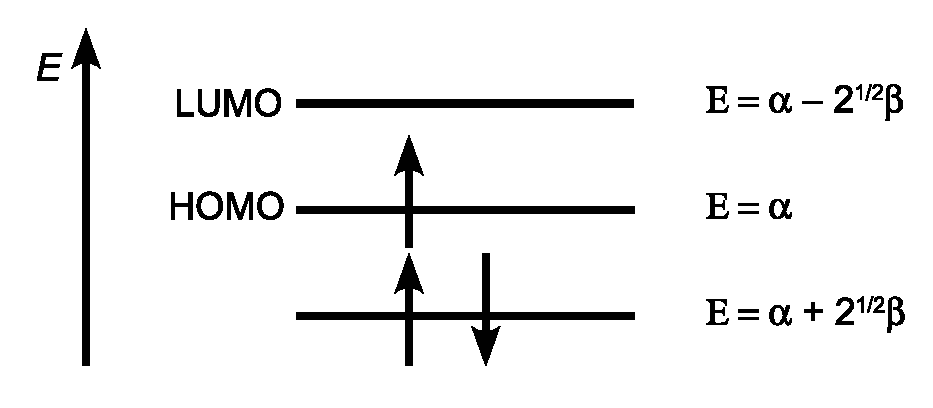
\includegraphics[scale=0.4]{huckelmo}
\end{figure}

\noindent
a) The energy difference between HOMO and LUMO orbitals is:

$$\Delta E = E_\textnormal{LUMO} - E_\textnormal{HOMO} = \alpha 
- \sqrt{2}\beta - \alpha = -\sqrt{2}\beta = -\sqrt{2}\times (-22,000
\textnormal{cm}^{-1})$$

$$\rightarrow \Delta E = 3.86 \textnormal{eV}~(320\textnormal{~nm})$$

\noindent
b) Next we calculate the coefficients $c_1, c_2$ and $c_3$ for the lowest
energy orbital:

\noindent
Here $E = (\alpha\pm\sqrt{2}\beta)$, which with $(\alpha - E)c_1 + \beta c_2 = 0$
gives $c_2 = \pm\sqrt{2}c_1$. Exactly the same way, equation
$\beta c_2 + (\alpha - E)c_3 = 0$ gives $c_2 = \pm\sqrt{2}c_3$.
Finally, normalization gives:
$c_1^2 + c_2^2 + c_3^2 = 1$ $\Rightarrow c_1^2 + (\pm\sqrt{2}c_1)^2
+ c_1^2 = 4c_1^2 \Rightarrow c_1 = \frac{1}{2}$ and by considering
$c_3$ the same way, we also get $c_3 = \frac{1}{2}$.\\

\noindent
Thus we have:

$$E = \alpha + \sqrt{2}\beta~\textnormal{with}~c_1 = \frac{1}{2},
c_2 = \frac{1}{\sqrt{2}}, c_3 = \frac{1}{2}$$
$$E = \alpha - \sqrt{2}\beta~\textnormal{with}~c_1 = \frac{1}{2},
c_2 = -\frac{1}{\sqrt{2}}, c_3 = \frac{1}{2}$$

\noindent
For $E = \alpha$, we have: $c_1 = \frac{1}{\sqrt{2}}, c_2 = 0, c_3 
= -\frac{1}{\sqrt{2}}$.\\

\noindent
The electron density on atom 1 can be obtained by squaring the atomic
basis function coefficients and weighing this by the number of electrons
on that orbital:\\

\noindent
Atom 1 ($i = 1$): $\sum_{j=1}^{3}|c_i^j|^2n_j = 
\left(\frac{1}{2}\right)^2\times 2 + \left(\frac{1}{\sqrt{2}}\right)^2
\times 1 + \left(\frac{1}{2}\right)^2\times 0 = 1$.\\
Atom 2 ($i = 2$): $\sum_{j=1}^{3}|c_i^j|^2n_j = 
\left(\frac{1}{\sqrt{2}}\right)^2\times 2 + 0^2
\times 1 + \left(-\frac{1}{\sqrt{2}}\right)^2\times 0 = 1$.\\
Atom 3 ($i = 3$): $\sum_{j=1}^{3}|c_i^j|^2n_j = 
\left(\frac{1}{2}\right)^2\times 2 + \left(-\frac{1}{\sqrt{2}}\right)^2
\times 1 + \left(\frac{1}{2}\right)^2\times 0 = 1$.\\

\noindent
The total charge (three $\pi$ electrons) is distributed evely to all three
atoms and therefore the partial charges on carbon atoms are equal.\\

\noindent
The bond orders can be valuated as follows:\\

\noindent
Bond between atoms 1 and 2 ($i = 1$ and $j = 2$):\\
$$\sum_{k=1}^{N_{MO}}c_i^k c_j^k n_k = 
\left(\frac{1}{2}\right)\left(\frac{1}{\sqrt{2}}\right)\times
2 + \left(\frac{1}{\sqrt{2}}\right)\times 0\times 1 
+ \left(\frac{1}{2}\right)\left(-\frac{1}{\sqrt{2}}\right)\times 0 
= \frac{1}{\sqrt{2}}$$
Bond between atoms 2 and 3 ($i = 2$ and $j = 3$):\\
$$\sum_{k=1}^{N_{MO}}c_i^k c_j^k n_k = 
\left(\frac{1}{\sqrt{2}}\right)\left(\frac{1}{2}\right)\times
2 + 0\times\left(-\frac{1}{\sqrt{2}}\right)\times 1
+ \left(-\frac{1}{\sqrt{2}}\right)\left(\frac{1}{2}\right)\times 0 
= \frac{1}{\sqrt{2}}$$

\noindent
The bond order is less than one ($\approx 0.707$), which indicates that
the bond is not very strong.\\

\hrule\vspace{0.5cm}
